\section{ChimeraX Rigid Fit protocol}
\label{app:chimeraRigidFit}%a040
Protocol designed to manually fit atomic structures to electron density maps in \scipion by using \chimera. If structure and map are quite close, e.g. after running $PowerFit$ protocol, automatic fitting is also possible. Fitted structures generated by using this protocol can be saved in \scipion after executing specific \chimera commands.
   
 \begin{itemize}
  \item Requirements to run this protocol and visualize results:
    \begin{itemize}
        \item \scipion plugin: \ttt{scipion-em-chimera}
    \end{itemize}
  \item \scipion menu:\\
   \ttt{Model building -> Rigid fitting} (\ffigure{fig:app_protocol_chimera_1} (A))
  
  \item Protocol form parameters (\ffigure{fig:app_protocol_chimera_1} (B)):
  
    \begin{figure}[H]
     \centering 
     \captionsetup{width=.7\linewidth} 
     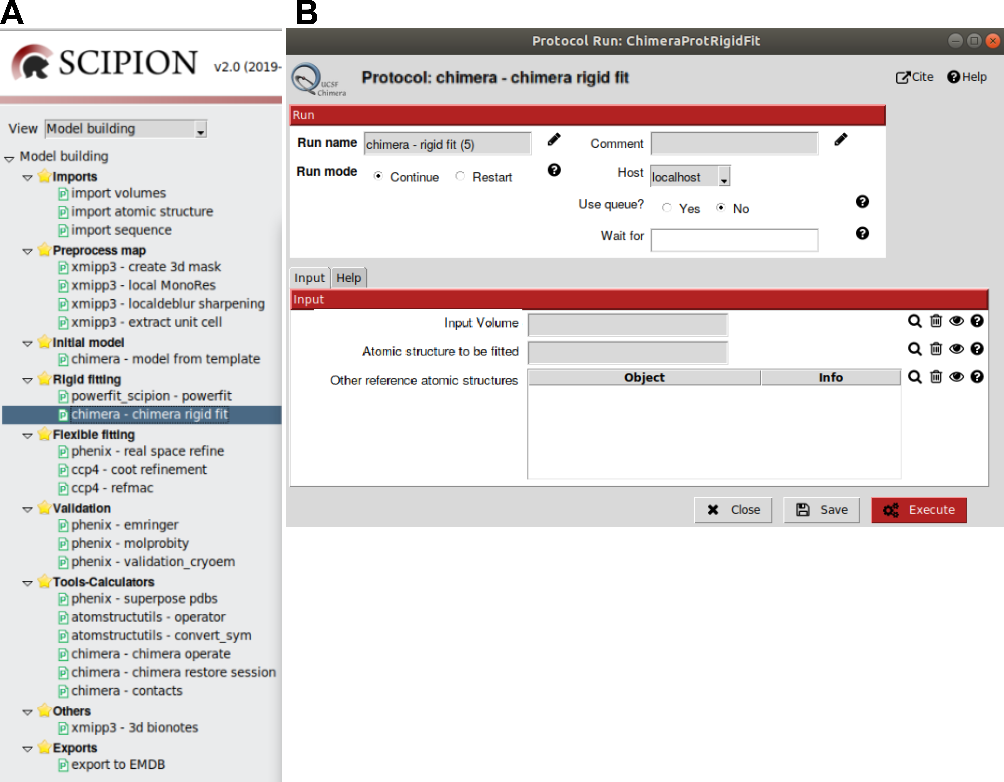
\includegraphics[width=0.90\textwidth]{Images_appendix/Fig116.pdf}
     \caption{Protocol \scommand{chimera rigid fit}. A: Protocol location in \scipion menu. B: Protocol form.}
     \label{fig:app_protocol_chimera_1}
    \end{figure}
    
    \begin{itemize}
     \item \ttt{Input} section

    \begin{itemize}
     \item \ttt{Input Volume}: Electron density map previously downloaded or generated in \scipion to fit the atomic structure.
     \item \ttt{Atomic structure to be fitted}: Atomic structure previously downloaded or generated in \scipion to be fitted to an electron density map.
     \item \ttt{Other reference atomic structures}: Atomic structures others than the $model$ that can help in the rigid body fitting process.
    \end{itemize}
    \item \ttt{Help} section
    
    This section contains \chimera commands required to save $models$ according to their reference volumes, which can also be saved if required. Remark that using \ttt{scipionwrite} command, \chimera session will be saved by default, without prejudice that it may be saved with \ttt{scipionss} command. \chimera sessions can be restored by using \scommand{chimera restore session} protocol.
    
    \end{itemize}

  \item Protocol execution:
  
  Adding specific map/structure label is recommended in \ttt{Run name} section, at the form top. To add the label, open the protocol form, press the pencil symbol at the right side of \ttt{Run name} box, complete the label in the new opened window, press OK and, finally, close the protocol. This label will be shown in the output summary content (see below). If you want to run again this protocol, do not forget to set to \ttt{Restart} the \ttt{Run mode}.\\
  Press the \ttt{Execute} red button at the form bottom.\\
  
  \chimera graphics window will be opened after executing the protocol. The electron density map and the atomic structure are shown. Main steps to complete the rigid body fitting are:
  \begin{itemize}
   \item If density map and atomic structure are quite close to each other:\\Go to \chimera main menu and select \ttt{Tools -> Volume -> Fit in Map}. A small \ttt{Fit in Map} window will be opened. Once atomic structure and electron density volume have been selected, fit them by clicking \ttt{Fit}. Press \ttt{Help} to consider different fitting options.
   \item If map and $model$ are far to each other, start the fitting process interactively activating and inactivating \chimera objects alternatively to finally get map and $model$ close enough to go to the previous step. 
   \item Save fitted $model$ regarding the electron density map by writing in \chimera command line:\\ \ttt{scipionwrite model \#n refmodel \#n saverefmodel 0/1}.\\Replace \ttt{\#n} by model numbers shown in \chimera \ttt{Model Panel}. Select \ttt{1} if you want to save the reference map or \ttt{0} otherwise, to avoid duplicate data unnecessarily.
   \item Close \chimera graphics window.
  \end{itemize}
  
  \item Visualization of protocol results:
  
    After executing the protocol, press \ttt{Analyze Results} and \chimera graphics window will be opened by default. Atomic structures and volumes are referred to the origin of coordinates in \chimera. To show the relative position of atomic structure and electron density volume, the three coordinate axes are represented; X axis (red), Y axis (yellow), and Z axis (blue) (\ffigure{fig:app_protocol_volume_3}). Coordinate axes, volume, and atomic structure are model numbers \ttt{\#0}, \ttt{\#1}, and \ttt{\#2}, respectively, in \chimera \ttt{Model Panel}.
   
  \item Summary content:
   \begin{itemize}
    \item If only the atomic structure has been saved by \ttt{scipionwrite} command:

   \begin{itemize}
     \item Protocol output (below \scipion framework):\\ \ttt{chimera - rigid fit -> ouputPdb\_01}; \ttt{AtomStruct (pseudoatoms=True/ False, volume=True/ False)}.\\Pseudoatoms is set to \ttt{True} when the structure is made of pseudoatoms instead of atoms. Volume is set to \ttt{True} when an electron density map is associated to the atomic structure.
     \item \ttt{SUMMARY} box:\\Produced files:\\chimeraOut0001.pdb\\we have some result
    \end{itemize}
    
   \item If both the atomic structure and its reference electron density map have been saved by \ttt{scipionwrite} command: 
   
   \begin{itemize}
     \item Protocol output (below \scipion framework):\\
      \ttt{chimera - rigid fit -> ouput3Dmap}; \ttt{Volume (x, y, and z dimensions, sampling rate)}.\\
      \ttt{chimera - rigid fit -> ouputPdb\_01}; \ttt{AtomStruct (pseudoatoms=True/ False, volume=True/ False)}.\\Pseudoatoms is set to \ttt{True} when the structure is made of pseudoatoms instead of atoms. Volume is set to \ttt{True} when an electron density map is associated to the atomic structure.
     \item \ttt{SUMMARY} box:\\Produced files:\\chimeraOut0001.pdb\\chimeraOut0001.mrc\\we have some result
    \end{itemize}
    
   \end{itemize} 
  
 \end{itemize}

